\documentclass[11pt, a4paper, oneside, pdftex]{research_paper}
%\usepackage[top=4.3cm, bottom=5.7cm, left = 3.74cm, right = 3.75cm]{geometry}
\setcounter{secnumdepth}{2}
\setcounter{tocdepth}{2}
\usepackage{titlesec}
\usepackage[dvips]{graphicx} 
\usepackage[
  bookmarks,
  bookmarksopen=true,
  pdftitle={ResearchPaper},
  linktocpage]{hyperref}


%\singlespacing
\usepackage{listings}

\begin{document}
\renewcommand{\bibname}{References}

\title{Improvements in classification and image recognition in Computer Vision}
\thispagestyle{empty}
\beforepreface
\titleformat{\chapter}{\normalfont\bfseries}{}{0pt}{\Large}
\titlespacing{\chapter}{0pt}{0pt}{40pt}

  
\section*{1. Introduction}
\hspace{30mm}    The advancements in computer hardware and machine learning algorithms have led to  big improvements in solving computer vision tasks such as image classification and image recognition, especially through the use of deep neural networks. \\
\null \hspace{30mm}	The use of artificial intelligence to solve such tasks has led to solutions in many domains and in different challenging situations (e.g. unsupervised or weakly-supervised learning). The recent advancements have also led to automated workflows, classification error minimization, faster data throughput and sometimes smaller network footprint, allowing computer vision processing to be present even in small, embedded devices. \\
\null \hspace{30mm}	Each year state-of-the-art results are surpassed either in very specific domains or even in general usage by creative algorithms or neural network architectures. In this report I will present some of the recent general-usage improvements in image recognition and image classification and will explore their applicability in embedded systems.

\section*{2. Selected papers}
\subsection*{Accepted papers}

\hspace{10mm} • \quad A Discriminative Channel Diversification Network for Image Classification - Krushi \\ \null \hspace{17mm} Patel, Guanghui Wang \\
\null \hspace{10mm} • \quad Semantic Clustering based Deduction Learning for Image Recognition and \\ \null \hspace{17mm} Classification - Wenchi Ma, Xuemin Tu, Bo Luo, Guanghui Wang \\
\null \hspace{10mm} • \quad Slim-RFFNet: Slim deep convolution random Fourier feature network for image \\ \null \hspace{17mm} classification - Tingting Wang, Bo Dong, Kaichun Zhang, Junbao Li, Lei Xu \\
\null \hspace{10mm} • \quad M-GCN: Brain-inspired memory graph convolutional network for multi-label image \\ \null \hspace{17mm} recognition - Xiao Yao, Feiyang Xu, Min Gu, Peipei Wang \\
\null \hspace{10mm} • \quad A Universal Representation Transformer Layer for Few-Shot Image Classification \\ \null \hspace{17mm} - Lu Liu, William Hamilton, Guodong Long , Jing Jiang , Hugo Larochelle


\subsection*{Rejected papers}
\hspace{10mm} •	\quad Discriminative Feature Mining and Enhancement Network for Low-resolution Fine- \\ \null \hspace{17mm} grained Image Recognition - Tiantian Yan; Haojie Li; Baoli Sun; Zhihui Wang; \\ \null \hspace{17mm} Zhongxuan Luo \\
\null \hspace{10mm} •\quad Deep collaborative multi-task network: A human decision process inspired model for \\ \null \hspace{17mm} hierarchical image classification – Yu Zhou, Xiaoni Li, Yucan Zhou, Yu Wang, \\ \null \hspace{17mm} Qinghua Hu, Weiping Wang \\
\null \hspace{10mm} • \quad Enhancing Few-Shot Image Classification with Unlabelled Examples – Peyman \\ \null \hspace{17mm} Bateni, Jarred Barber, Jan-Willem van de Meent, Frank Wood \\
\null \hspace{10mm} • \quad SAR image classification based on multi-feature fusion decision convolution neural \\ \null \hspace{17mm} network - Liang Guo \\
\null \hspace{10mm} • \quad	Visual vs internal attention mechanisms in deep neural networks for image \\ \null \hspace{17mm} classification and object detection - Abraham Montoya Obeso, Jenny Benois-Pineau, \\ \null \hspace{17mm} Mireya Sarai Garcia Vasquez, Alejandro Alvaro Ramirez Acosta \\
\null \hspace{10mm} • \quad	Performance comparison of CNN, QNN and BNN deep neural networks for real-time \\ \null \hspace{17mm} object detection using ZYNQ FPGA node – V.R.S. Mani, A. Saravanaselvan, N. \\ \null \hspace{17mm} Arumugam \\
\null \hspace{10mm} • \quad	Class-Balanced Active Learning for Image Classification - Javad Zolfaghari Bengar, \\ \null \hspace{17mm} Joost van de Weijer, Laura Lopez Fuentes, Bogdan Raducanu \\
\null \hspace{10mm} • \quad	Robust Semi-supervised Federated Learning for Images Automatic Recognition in \\ \null \hspace{17mm} Internet of Drones - Zhe Zhang, Shiyao Ma, Zhaohui Yang, Zehui Xiong, Jiawen \\ \null \hspace{17mm} Kang, Yi Wu, Kejia Zhang, Dusit Niyato \\
\null \hspace{10mm} • \quad High-Performance FPGA-based Accelerator for Bayesian Neural Networks - \\ \null \hspace{17mm} Hongxiang Fan, Martin Ferianc, Miguel Rodrigues, Hongyu Zhou, Xinyu Niu, Wayne \\ \null \hspace{17mm} Luk \\
\null \hspace{10mm} • \quad FPGA-optimized Hardware acceleration for Spiking Neural Networks - Alessio \\ \null \hspace{17mm} Carpegna, Alessandro Savino, Stefano Di Carlo


\section*{3. Accepted papers presentation}

\hspace{20mm}•\hspace{3mm}	A Discriminative Channel Diversification Network for Image Classification - Krushi Patel, Guanghui Wang \\
\null \hspace{30mm}	The paper proposes a new channel diversification block, which consists in some additional layers in a specific configuration,  which can be added near the end of any CNN in order to make it concentrate on the diverse and significant channels at the same time. By doing this, information can be extracted in a more homogenous manner from the whole picture. \\
\goodbreak
\begin{figure}[!h]
    \centering
    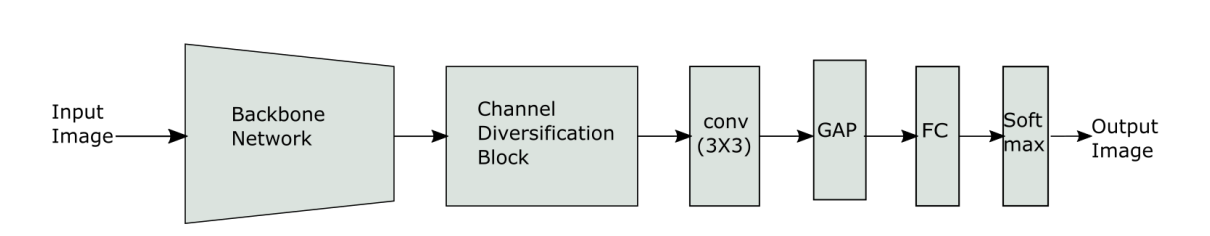
\includegraphics[width=0.9\linewidth]{figures/image_1}
    \caption{The architecture of the classification network with the channel diversification network}
    \label{fig:figure1}\cite{1}
\end{figure}
\null \hspace{30mm}	This type of channel attention mechanisms have been proven to increase the accuracy in image classification tasks, but also come with additional model complexity and computation cost. The proposed block is both light-weight and effective, increasing the accuracy of baseline models more than the other state-of-the-art attention mechanisms such as the squeeze and excitation block, the spatially attentive output layer or the attention branch network in most situations, while providing an overhead of the number of parameters of only a few percentages, smaller than the other methods. \\
\null \hspace{30mm}	The method was tested on 7 different architectures and considering its generality and light-weight nature it looks promising for enhancing image classification accuracy in embedded implementations. \\

\hspace{20mm}•\hspace{3mm}	Semantic Clustering based Deduction Learning for Image Recognition and Classification - Wenchi Ma, Xuemin Tu, Bo Luo, Guanghui Wang \\
\null \hspace{30mm}	The paper proposes an algorithm of semantic clustering based on deduction learning, by mimicking the learning and thinking process of the human brain. The algorithm is applied at the beginning and end of CNNs,. By doing the high-level clustering (e.g.: cat class and dog class in a cluster, car class  and boat class in another cluster) in the semantic space the model is able to deduce the relations among various classes for a better learning. \\
\null \hspace{30mm}	The algorithm also has a penalizing component: by doing a semantic prior random search for the opposite labels it ensures the smooth distribution of the clustering. \\
\goodbreak
\begin{figure}[!h]
    \centering
    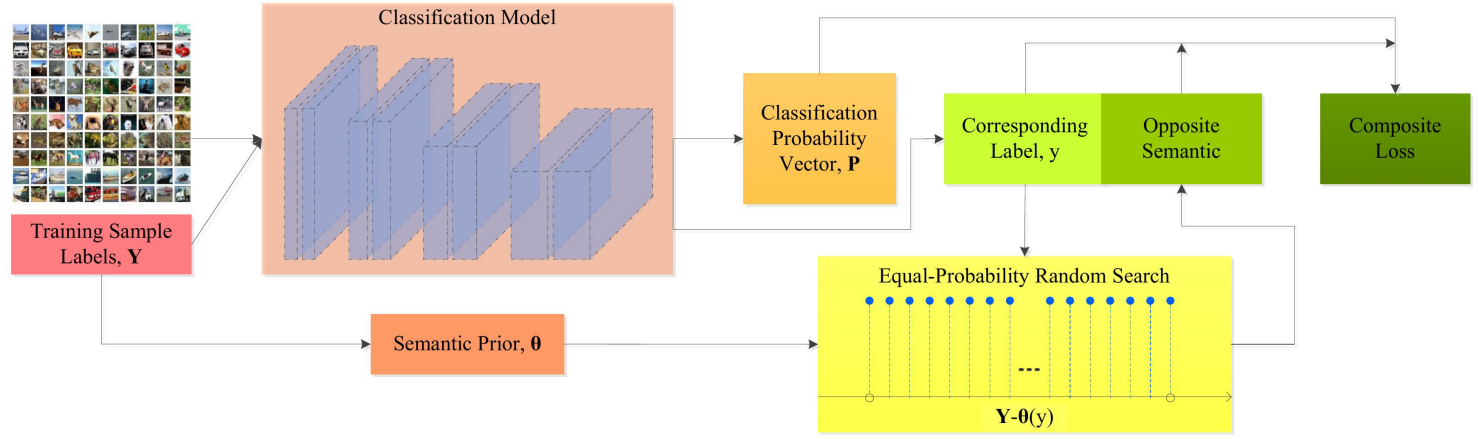
\includegraphics[width=0.9\linewidth]{figures/image_2}
    \caption{ An overview of the proposed method. Semantic prior based random search is used
to produce opposite semantic in order to form the composite loss function, guiding the model to
form semantic colonies}
    \label{fig:figure2}\cite{2}
\end{figure}  
\null \hspace{30mm}	Using the algorithm as a plug-in module in tasks implying supervised learning, few-shot learning, zero-shot learning or semi-supervised learning provides an increase in classification accuracy on classical and state-of-the-art classifiers. The method is also tested to be resilient to noisy labeling and light-weight, thus being suitable for embedded implementation. \\

\hspace{20mm}•\hspace{3mm}	Slim-RFFNet: Slim deep convolution random Fourier feature network for image classification - Tingting Wang, Bo Dong, Kaichun Zhang, Junbao Li, Lei Xu \\
\null \hspace{30mm}	The paper proposes a 28 layer RFFNet (random Fourier feature network) which outperforms current state-of-the-art kernel learning methods. The network also achieves a trade-off between accuracy and latency, while mentaining a small memory footprint, being thus suitable for resource-constrained embedded devices. \\
\null \hspace{30mm}	The authors identify feature concatenation and global average pooling as the best methods to bypass connections and downsample them. They also use quantization in order to reduce the data size from float32 to int8 where possible. This slightly reduces the overall accuracy but greatly improves latency time and memory footprint. \\
\null \hspace{30mm}	This architecture was tested on 1 Intel and 2 ARM devices and it performed similarly, slightly better on the ARM devices. On 96x96 resolution images the model size was ~63 MB without quantization or ~ 15 MB with quantization, while the inference latency was 22 ms or lower without quantization and 11 ms or lower with quantization. \\
\null \hspace{30mm}	One limitation of this proposed network is that according to Bochner’s theorem, it can only use the translation invariant kernel. Meanwhile, non-translation invariant kernels have better performance in more special fields. Also the network needs to be retrained when classifying cross-domain data. \\

\hspace{20mm}•\hspace{3mm}	M-GCN: Brain-inspired memory graph convolutional network for multi-label image recognition - Xiao Yao, Feiyang Xu, Min Gu, Peipei Wang \\
\null \hspace{30mm}	The paper proposes a neural network architecture inspired by the hippocampal circuit and memory mechanism of human brain, named Memory Graph Convolutional Network (M-GCN). The network has short-term and long-term memory modules, learning complex semantic enhancement and suppression. \\
\null \hspace{30mm}	The purpose of this brain-inspired neural network is to enhance multi-label classification by utilizing the semantics between objects. The model combines the efficient semantic recognition mechanism of CNNs and the direct semantic correlation of GANs. \\
\null \hspace{30mm}	The method performs overall better than other state-of-the-art multi-label image recognition networks such as SSGRL (Semantic-Specific Graph Representation Learning), MCAR (Multi-Class Attentional Regions) or HCP (Hypotheses-CNN-Pooling). \\
\null \hspace{30mm}	The proposed method was implemented using PyTorch on a powerful computer. Judging by the implementation present on GitHub, it seems unlikely that it would be suitable for embedded systems, but could serve as inspiration for a light-weight brain-inspired neural network for multi-label image recognition, if combined with other optimization techniques, like quantization. \\

\hspace{20mm}•\hspace{3mm}	A Universal Representation Transformer Layer for Few-Shot Image Classification - Lu Liu, William Hamilton, Guodong Long , Jing Jiang , Hugo Larochelle \\
\null \hspace{30mm}	This research treats the problem of multi-domain few-shot image classification. Few-shot image classification means the number of images available for training is very small. Since machine learning systems generally improve with the availability of more data, a natural assumption is that few-shot learning systems should benefit from leveraging data across many different tasks and domains, even if each individual task has limited training data available. \\
\null  \hspace{30mm} This paper improves the state-of-the-art SUR (Selecting Universal Representation) multi-domain few-shot classification algorithm, which relies on a so-called universal representation. It can be achieved by extracting from a collection of pre-trained and domain-specific neural network backbones. It prescribes a hand-crafted feature-selection procedure to infer how to weight each backbone for each task, and produces an adapted representation for each one. Yet there is no cross-domain generalization, which could be beneficial in such low data problems. \\
\null \hspace{30mm}	The proposed method, URT (Universal Representation Transformer) layer, can effectively transform a universal representation into task-adapted representations. It uses an attention mechanism to learn to retrieve or blend the appropriate backbones to use for each task. By training this layer across few-shot tasks from many domains, it can support transfer across these tasks. \\
\null \hspace{30mm}	By using the URT layer on top of SAR’s universal representation there are achieved new state-of-the-art results on the Meta-Dataset. \\
\null \hspace{30mm}	As the URT layer is relatively light-weight, the problem of it being embedded-friendly depends on the underlying SAR architecture.

\section*{4. Conclusions}

\hspace{30mm} By examining multiple state-of-the-art research papers on the topic of computer vision, with the focus on image recognition and image classification, various approaches have been identified for different applicability scenarios: from unsupervised learning deep neural networks all the way to supervised systems, from plug-in modules created to enhance the performance of other state-of-the-art networks up to new, complete,  deep neural network architectures. The generality of each one of the proposed solutions allows versatile applicability and more important, most of the solutions seem applicable also on embedded systems, as detailed in the last paragraph of each paper presentation.

\begin{thebibliography}{24}

\bibitem{1}	K. PATEL, G. WANG, \textit{A Discriminative Channel Diversification Network for Image Classification}, Pattern Recognition Letters \textbf{153}, pp. 176-182, Jan 2022.
\bibitem{2}	W. MA, X. TU, B. LUO, G. WANG, \textit{Semantic Clustering based Deduction Learning for Image Recognition and Classification}, Pattern Recognition Letters \textbf{124}, Apr 2022.
\end{thebibliography}
\end{document}
